\newpage
\section{Conservation of Momentum}
\begin{definition}
    Two or more objects interact and \textbf{exert forces from each other}. 
    The forces in the interaction are a Newton's Third Law pair of forces (ie $\vec{F_{A/B}} = -\vec{F_{B/A}}$)
\end{definition}

\subsection{Equation}
Consider a person standing on any icy surface throws a heavy object horizontally:\\

\begin{center}
    FBD for the person (Left) and the object (Right)
\end{center}

\begin{figure}[h!]
    \centering
    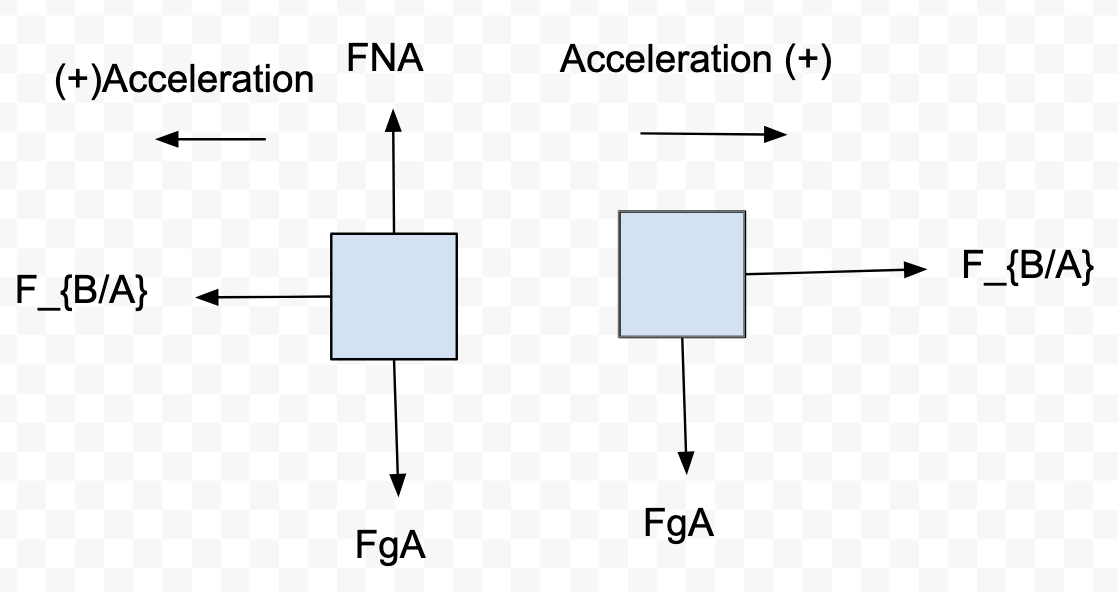
\includegraphics[width=0.7\textwidth]{graph/3.7.1.png}
    \caption{We will assume that the interaction forces are essentially the net force acting on the object}
\end{figure}

Equation for the object A:
\begin{align}
    \sum \vec{F_{A}} &= m_A \vec{a_A} \nonumber \\
    \vec{F_{B/A}} &= m_A \vec{a_A} \nonumber \\
    \vec{F_{B/A}} &= m_A\frac{\vec{v_{fA}} - \vec{v_{iA}}}{\Delta t_A} \label{eq: eq1}
\end{align}

Equation for the object B:
\begin{align}
    \sum \vec{F_{B}} &= m_B \vec{a_B} \nonumber \\
    \vec{F_{A/B}} &= m_B \vec{a_B} \nonumber \\
    \vec{F_{A/B}} &= m_B\frac{\vec{v_{fB}} - \vec{v_{iB}}}{\Delta t_B} \label{eq: eq2}
\end{align}

\begin{lemma}
    From Newton's third law, we know $\vec{F_{A/B}} + \vec{F_{B/A}} = 0$
\end{lemma}

We add \ref{eq: eq1} and \ref{eq: eq2} together:
\begin{align*}
    m_A\frac{\vec{v_{fA}} - \vec{v_{iA}}}{\Delta t_A} + m_B\frac{\vec{v_{fB}} - \vec{v_{iB}}}{\Delta t_B} &= 0
\end{align*}

We know the time for both object should be the same.
\begin{align}
    m_A \vec{v_{fA}} + m_B \vec{v_{fB}} &= m_A \vec{v_{iA}} + m_B \vec{v_{iB}} \nonumber\\
    \vec{P_{A2}} + \vec{P_{B2}} &= \vec{P_{A1}} + \vec{P_{B1}} \label{eq: eq3}
\end{align}

\ref{eq: eq3} is the law of \textbf{Conservation of Momentum}

Always write this line at the beginning of your analysis:

\begin{definition} [The Law of Conservation of Momentum]\label{def: de1}
     The total momentum of a system of objects after an interaction is 
    \textbf{equal} to the total momentum of the system before the interaction. 
\end{definition}

According to \ref{def: de1}, the total momentum of the system is \textbf{constant throughout}
the interaction. \\

This law assumes that any other force that could \textbf{accelerate} objects in the system during the 
interaction is \textbf{negligible}.
